% !TEX root = ../thesis-example.tex
%
\section{Additional Coloring Operations}

Finally we have created the best possible recreation of a VR actor inside the 
virtual reality scene. Now we can follow up with post effects on the video feed 
to fit it to a better degree into the environment. This can be done with 
regular coloring operations, like hue rotation, brightness, contrast and 
saturation procedures on the video alone. It gives a content producer direct 
enhancing tools which would be given by Unitys' post effects stack but are 
unavailable due to the nature of this render pipeline.

\begin{figure}[htb]
	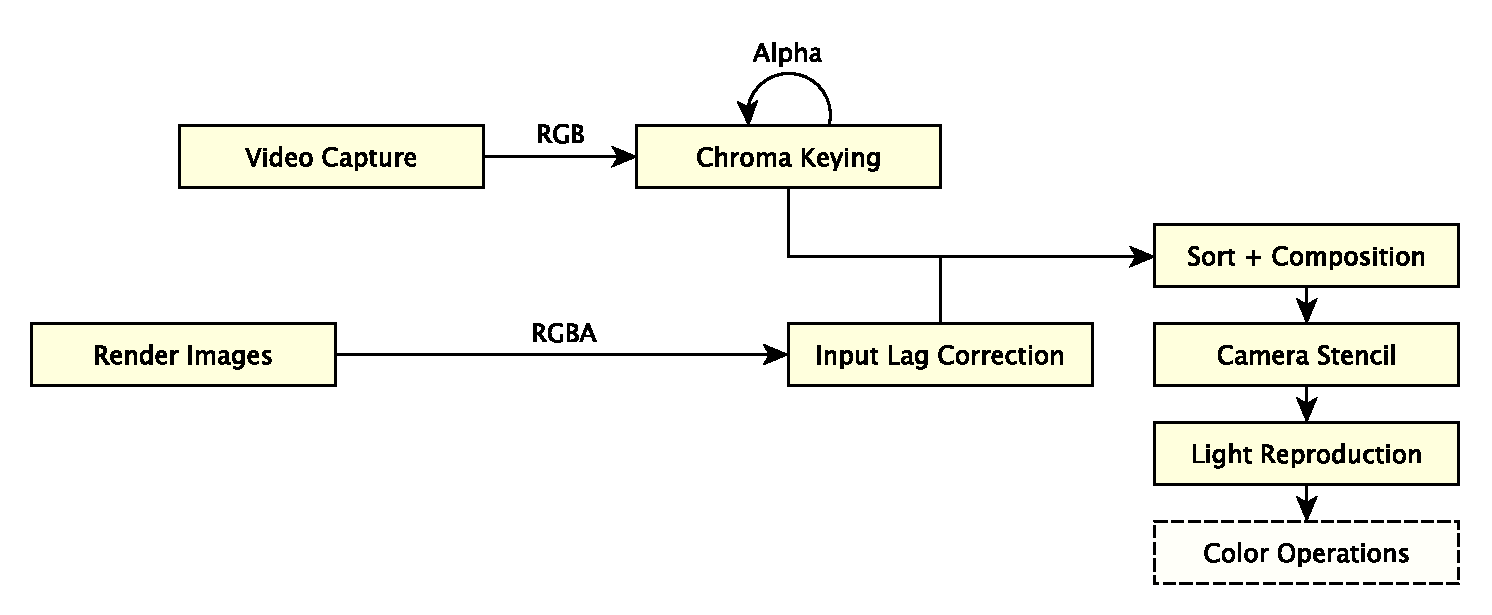
\includegraphics[width=\textwidth]{_raw_resources/pipeline_steps/4_8_color.pdf}
	\caption{Initial step upon receiving the camera image}
	\label{fig:steps:recolor}
\end{figure}

\subsection{Color spill removal \& Recoloring}

The green box as background spills - so to say - its green color on the actor 
to a certain degree. With proper lightning setups it is possible to mitigate 
its effects but color retouching is always a necessity. \textbf{YCgCo} is, 
again, good enough to perform this color operation, thanks to its color 
decoupling properties. By splitting a RGB image into YCgCo $C_{Input}$ (see 
equation \eqref{eq:ycgco:transformation}) and then shifting towards the 
anti-color of the key color $C_{Key}$ for a factor weight $W \in [0, 1]$:

\eq{eq:retouch:spill:1}{
	R = \frac{C_{Key Cg, Co} \cdot C_{Input Cg, Co}}{C_{Key Cg, Co} \cdot 
	C_{Key Cg, Co}}
}

\eq{eq:retouch:spill:2}{
	\begin{bmatrix}
		Y  \\
		Cg \\
		Co \\
	\end{bmatrix}
	= 
	\begin{bmatrix}
		Y \\
		C_{Key Cg} * (R + 0.5) * W \\
		C_{Key Co} * (R + 0.5) * W
	\end{bmatrix}
}

\todo[inline]{"proper lightning setup" would be something for the appendix}

Since this is a linear operation, it does not consider more apparent color 
spill around an actors edges - it slightly removes a green undertone to make it 
look more natural and fitting in this scene.

Additionally we can apply a hue color rotation by using Rodrigues' rotation 
formula to make changes to the overall tint of an image, shifting a color $C_I$ 
180 degrees forwards or backwards with a factor $H \in (-\pi, \pi]$ to yield a 
color $C_F$:
\eq{eq:retouch:hue}{
	C_F = C_I \cos(H) + (0.57735 \times C_I) \sin(H) + 0.57735 (k \cdot C_I) 
	(1 - \cos(H))
}
\todo[inline]{sourcing on 0.57735 needed}

With that we can achieve a more natural looking video feed that integrates well 
into any given scene. Allowing for color-shifting degrades the signal but 
allows for a more fitting composition between an actor and his surrounding 
virtual reality scenery.

\subsection{Brightness, Contrast and Saturation}

Additionally, to give a user full control over image composition, we have a 
brief look at other linear image transformations to give good control over the 
video feed, which are brightness, contrast and saturation operations:

\begin{lstlisting}
	# aint nobody got time for that - here's HLSL
	# brightness:
	rgb = saturate(rgb + Brightness)
	# Contrast
	rgb = saturate((rgb - 0.5f) * Contrast + 0.5)
	# saturation:
	# - calc the most color-intense point
	# - then simply mix both colors
	half l = dot(rgb, half4(0.2126, 0.7152, 0.0722))
	rgb = saturate(lerp(l, rgb, _Saturation));
\end{lstlisting}


